% Kempe chains (generated by figs_c1ch07.py).
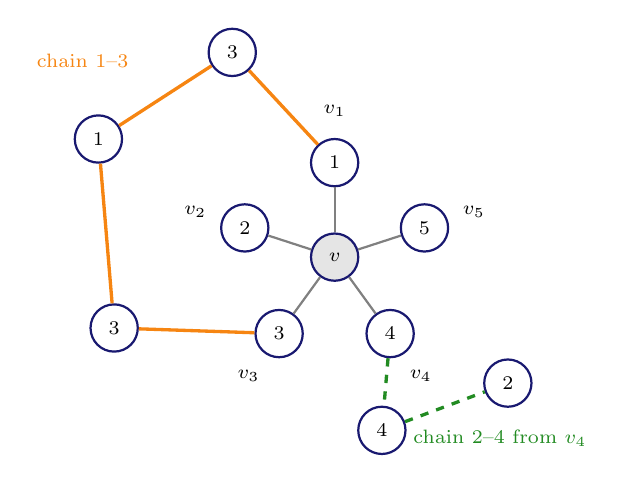
\begin{tikzpicture}[x=1cm,y=1cm,n/.style={circle,draw=MidnightBlue,thick,fill=white,inner sep=1pt,minimum size=6mm,font=\scriptsize}]
\node[n,fill=gray!20] (v) at (0,0) {$v$};
\node[n] (v1) at (0.000,1.200) {$1$};
\draw[thick,gray] (v) -- (v1);
\node[n] (v2) at (-1.141,0.371) {$2$};
\draw[thick,gray] (v) -- (v2);
\node[n] (v3) at (-0.705,-0.971) {$3$};
\draw[thick,gray] (v) -- (v3);
\node[n] (v4) at (0.705,-0.971) {$4$};
\draw[thick,gray] (v) -- (v4);
\node[n] (v5) at (1.141,0.371) {$5$};
\draw[thick,gray] (v) -- (v5);
\node[n] (a) at (-1.3,2.6) {$3$}; \node[n] (b) at (-3.0,1.5) {$1$}; \node[n] (c) at (-2.8,-0.9) {$3$};
\draw[very thick,BurntOrange] (v1) -- (a) -- (b) -- (c) -- (v3);
\node[n] (d) at (0.6,-2.2) {$4$}; \node[n] (f) at (2.2,-1.6) {$2$};
\draw[very thick,ForestGreen,dashed] (v4) -- (d) -- (f);
\node[font=\scriptsize,BurntOrange] at (-3.2,2.5) {chain $1$--$3$};
\node[font=\scriptsize,ForestGreen] at (2.1,-2.3) {chain $2$--$4$ from $v_4$};
\node[font=\scriptsize] at (0.000,1.860) {$v_1$};
\node[font=\scriptsize] at (-1.769,0.575) {$v_2$};
\node[font=\scriptsize] at (-1.093,-1.505) {$v_3$};
\node[font=\scriptsize] at (1.093,-1.505) {$v_4$};
\node[font=\scriptsize] at (1.769,0.575) {$v_5$};
\end{tikzpicture}
